\chapter{RESULTADOS E DISCUSSÃO}
\label{chapter:resultados}

Este capítulo apresenta os resultados da simulação do robô com o motor a 30 rpm no sentido anti-horário, durante 8 s, para o modelo do Capítulo \ref{chapter:modelo} com os parâmetros inerciais do Capítulo \ref{chapter:inercia}. Os pontos escolhidos para acompanhar o deslocamento são o centro de massa do robô e a ponta superior de cada braço (a mão).

\section{Movimento das Alavancas}
\label{sec:res_alavancas}

A \ref{fig:alavancas_res} mostra o ângulo das duas alavancas e suas derivadas ao longo de uma volta da manivela (2 s), calculados pelas Equações \ref{eq:phi} e \ref{eq:dphi}. Os braços oscilam em oposição de fase entre $-11,4^\circ$ e $+11,4^\circ$, com velocidade angular máxima de 0,77 rad/s e aceleração angular máxima de 2,34 rad/s$^2$. O movimento não é senoidal puro: a fenda e o pino fazem com que o curso em um sentido dure mais que no outro (cerca de 203$^\circ$ de manivela contra 157$^\circ$).

\begin{figure}[H]
\begin{center}
 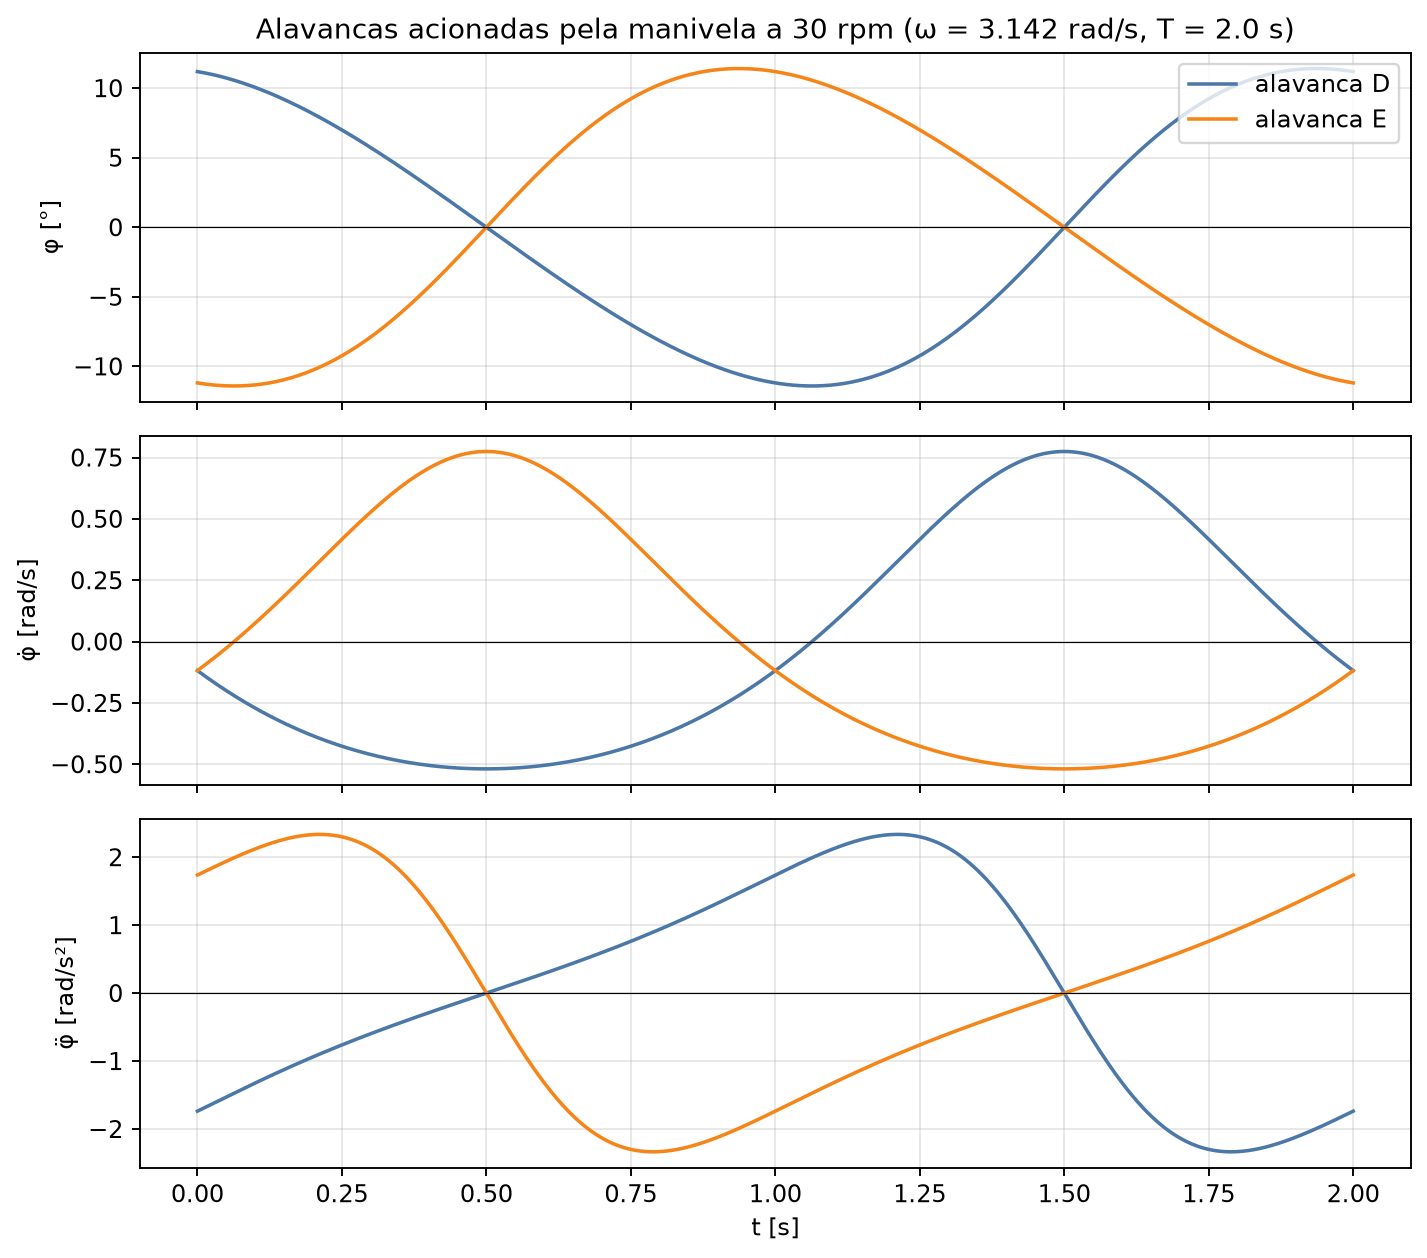
\includegraphics[width=12.5cm]{alavancas.png}
\caption{\label{fig:alavancas_res}- Ângulo, velocidade angular e aceleração angular das alavancas D e E para a manivela a 30 rpm.}
\end{center}
\end{figure}

\section{Deslocamento do Centro de Massa e das Mãos}
\label{sec:res_deslocamento}

A \ref{fig:deslocamento_res} mostra o avanço do centro de massa e da ponta das duas mãos, positivo para a frente, comparado com a reta da cinemática pura (Equação \ref{eq:vcin}), além dos ângulos do chassi e das pernas e da força vertical da corda sobre o gancho engatado. As linhas pontilhadas marcam as trocas de mão, listadas na \ref{tab:trocas}. Os valores numéricos da simulação estão reunidos na \ref{tab:resultados}.

\begin{figure}[H]
\begin{center}
 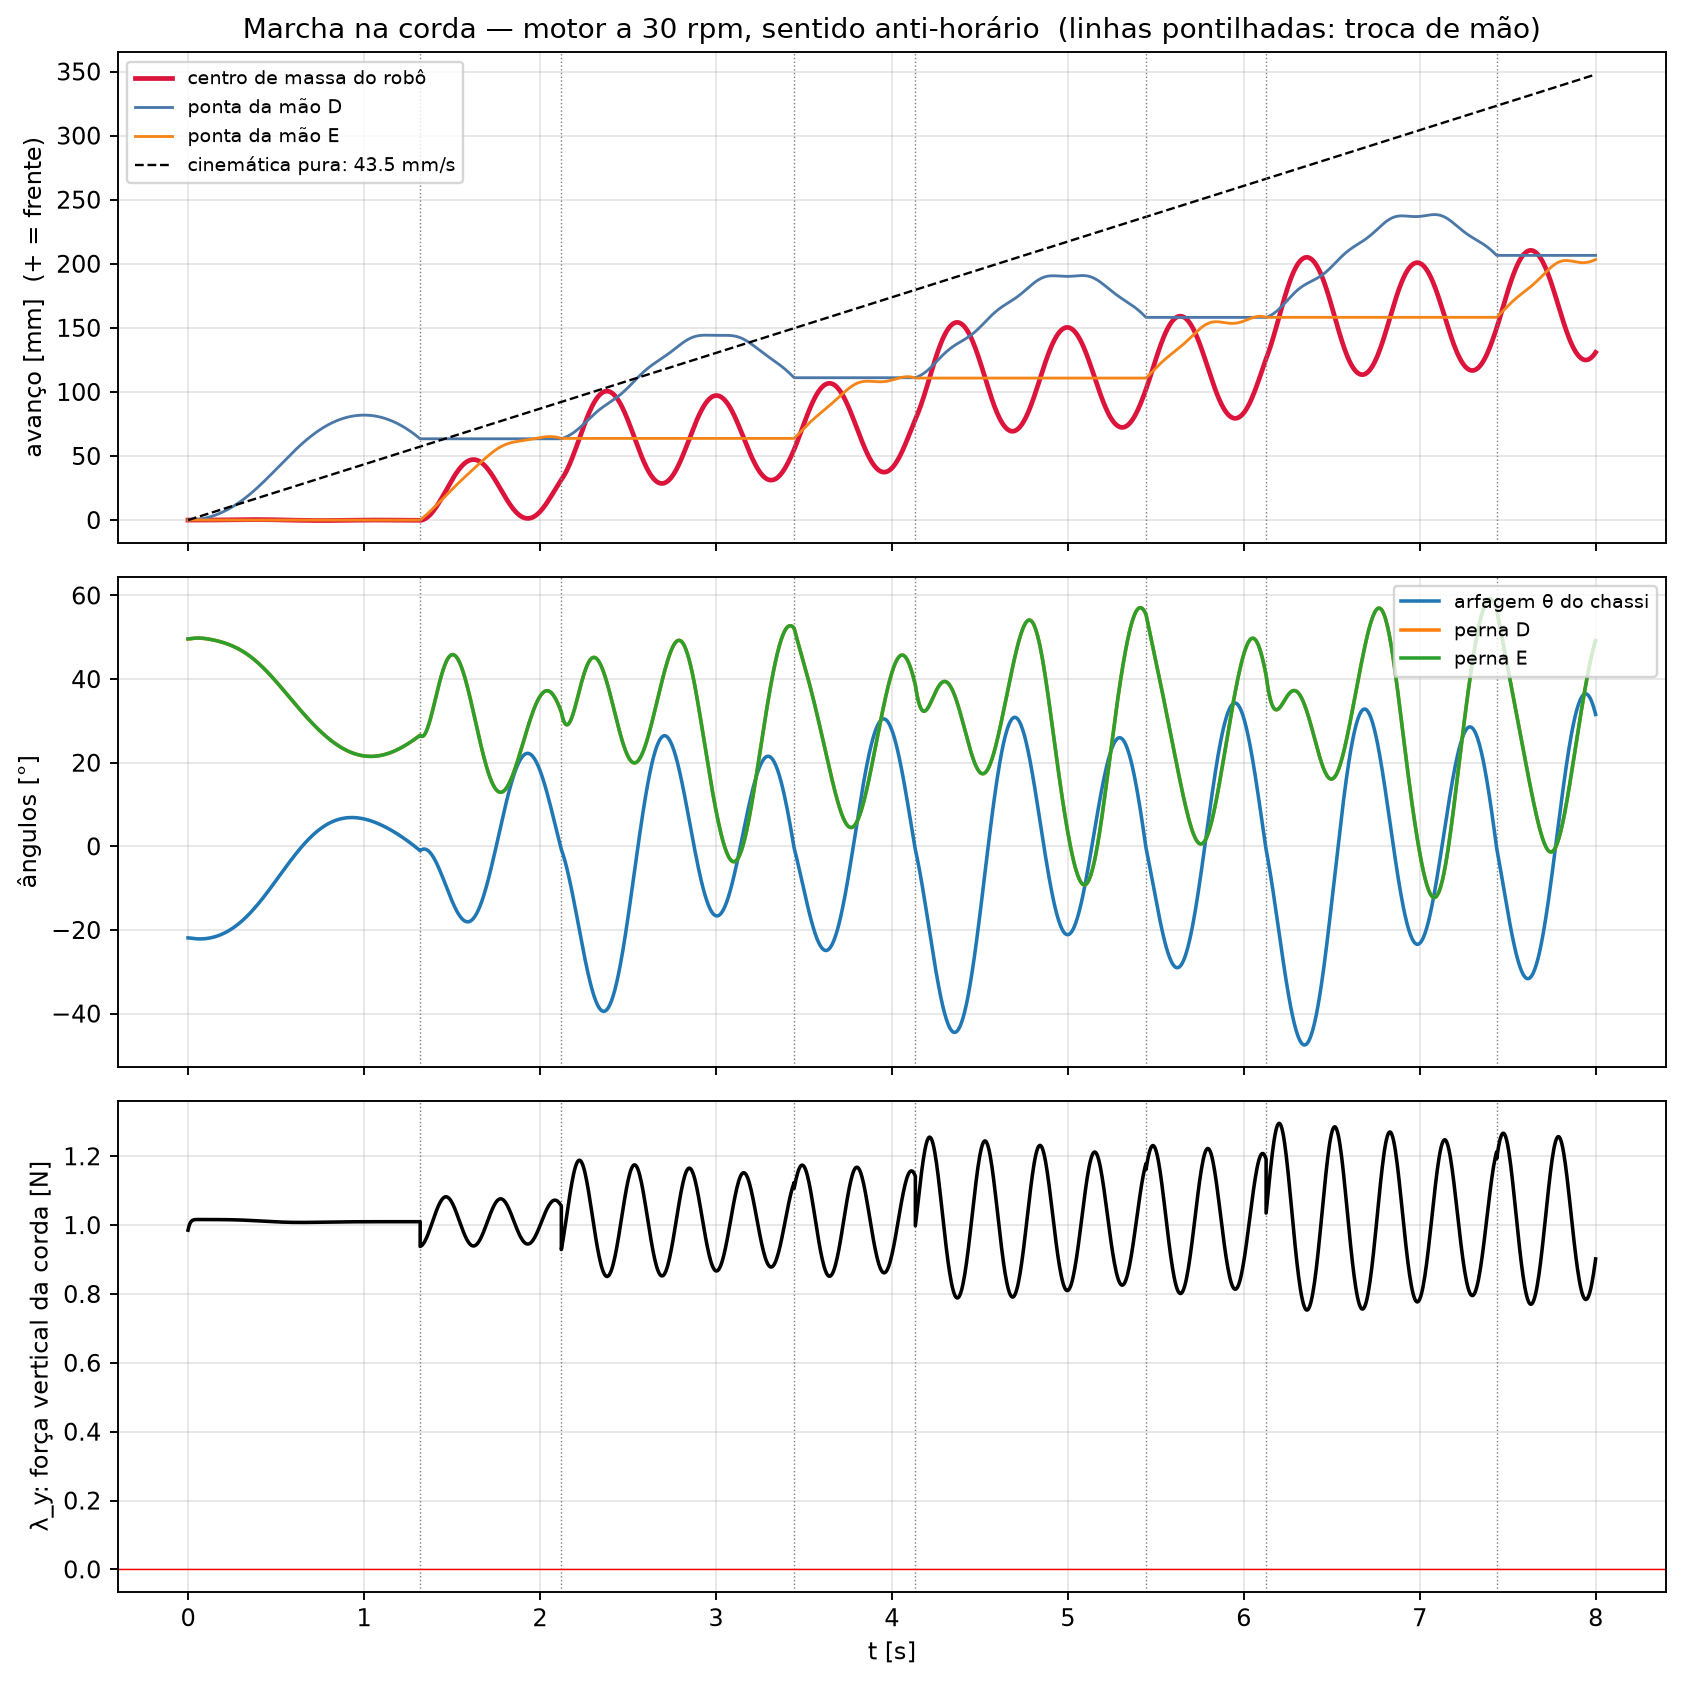
\includegraphics[width=14cm]{deslocamento.png}
\caption{\label{fig:deslocamento_res}- Avanço do centro de massa e das mãos, ângulos do chassi e das pernas e força vertical da corda ($c_{ch}=10^{-4}$ N$\cdot$m$\cdot$s/rad).}
\end{center}
\end{figure}

\begin{table}[H]
\centering
\caption{\label{tab:resultados}- Resultados da simulação (8 s, 30 rpm, anti-horário).}
\vspace*{.1cm}
\begin{tabular}{|l|c|}
\hline
\textbf{Grandeza} & \textbf{Valor} \\
\hline
Avanço do centro de massa & 130,8 mm \\
\hline
Avanço da ponta da mão D & 206,5 mm \\
\hline
Avanço da ponta da mão E & 203,3 mm \\
\hline
Velocidade média na última volta & 22,6 mm/s \\
\hline
Limite da cinemática pura & 43,5 mm/s \\
\hline
Razão entre as duas velocidades & 52\,\% \\
\hline
Variação da altura do centro de massa & 18,0 mm \\
\hline
Arfagem máxima do chassi & 47,5$^\circ$ \\
\hline
Ângulo máximo das pernas em relação ao chassi & 59,2$^\circ$ \\
\hline
Força vertical da corda sobre o gancho & de 0,75 a 1,30 N (peso: 1,01 N) \\
\hline
Número de trocas de mão & 7 \\
\hline
Energia máxima dissipada em um impacto & 1,5 mJ \\
\hline
\end{tabular}
\end{table}

O centro de massa avançou 130,8 mm em 8 s e as mãos avançaram 206,5 mm e 203,3 mm, de modo que o robô caminha para a frente, como esperado para a manivela no sentido anti-horário. A velocidade média na última volta foi de 22,6 mm/s, cerca de 52\,\% do limite da cinemática pura (43,5 mm/s). Esse limite supõe que o chassi não balança e que cada mão engata assim que a anterior termina o curso; na simulação, o gancho só engata quando sua ponta sobe até a corda, o que ocorre de 0,1 s a 0,4 s depois do instante em que a fase da manivela troca a mão desejada (\ref{tab:trocas}), e esse atraso, mais o curso perdido em cada espera, reduz a velocidade média.

\begin{table}[H]
\centering
\caption{\label{tab:trocas}- Trocas de mão: instante do engate, mão que engata, instante da troca da mão desejada, atraso e energia dissipada no impacto.}
\vspace*{.1cm}
\begin{tabular}{|c|c|c|c|c|}
\hline
\textbf{Engate (s)} & \textbf{Mão} & \textbf{Troca desejada (s)} & \textbf{Atraso (s)} & \textbf{Energia (mJ)} \\
\hline
1,32 & D & 1,00 & 0,32 & $-$0,01 \\
\hline
2,12 & E & 2,00 & 0,12 & 0,41 \\
\hline
3,44 & D & 3,00 & 0,44 & 0,00 \\
\hline
4,13 & E & 4,00 & 0,13 & 1,06 \\
\hline
5,44 & D & 5,00 & 0,44 & 0,02 \\
\hline
6,13 & E & 6,00 & 0,13 & 1,47 \\
\hline
7,44 & D & 7,00 & 0,44 & 0,05 \\
\hline
\end{tabular}
\end{table}

O mecanismo do avanço pode ser lido na \ref{fig:deslocamento_res}. Enquanto o robô está pendurado por uma mão, o centro de massa tende a ficar logo abaixo do gancho (equilíbrio do pêndulo), de modo que o curso do braço em relação ao chassi apenas altera a arfagem. É na troca de mão que o avanço ocorre: o novo gancho engata, em média, cerca de $S=43,5$ mm à frente na corda (curso da mão em relação ao chassi), e o robô balança para a frente sob a ação da gravidade em direção ao novo equilíbrio. Isso explica o aspecto em degraus da curva da mão e o balanço do centro de massa em torno da tendência média.

\section{Trajetórias, Ângulos e Forças}
\label{sec:res_traj}

A \ref{fig:trajetorias_res} mostra as trajetórias do centro de massa e das mãos no plano $x$--$y$. A mão engatada fica sobre a corda, e a mão livre descreve arcos acima e abaixo dela. O centro de massa permanece em média 82 mm abaixo da corda e oscila verticalmente por 18,0 mm. O chassi balança com amplitude de até 47,5$^\circ$ e as pernas, com amplitude de até 59,2$^\circ$ em relação ao chassi, que inclui o ângulo inicial de equilíbrio. A força vertical da corda sobre o gancho engatado variou entre 0,75 N e 1,30 N em torno do peso de 1,01 N e foi sempre positiva, ou seja, a corda nunca precisou empurrar o gancho para baixo, o que é coerente com a hipótese de contato unilateral.

\begin{figure}[H]
\begin{center}
 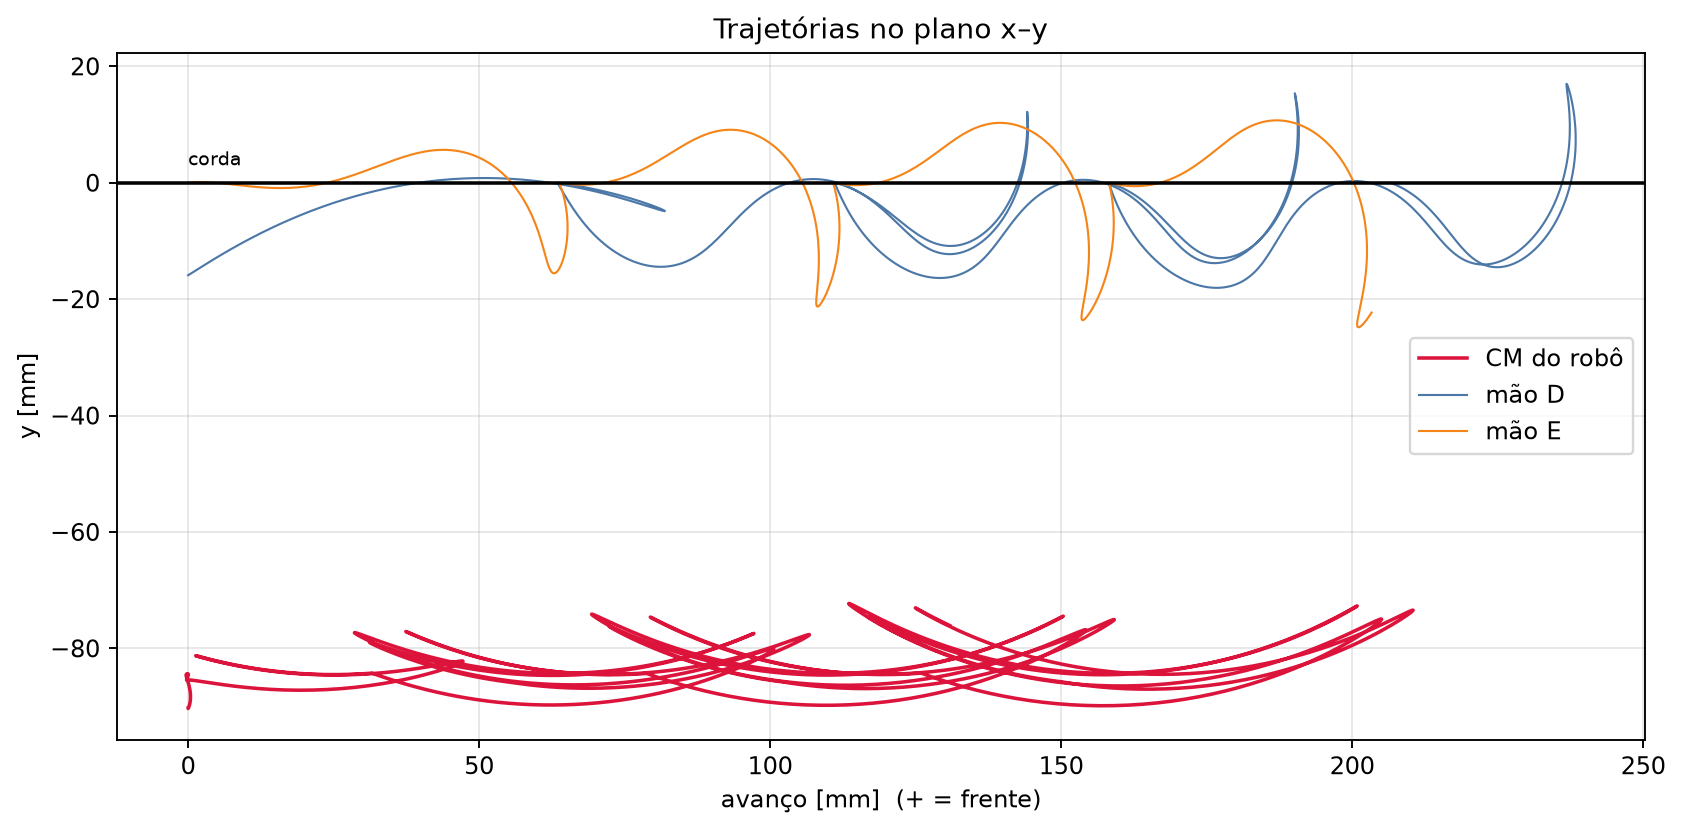
\includegraphics[width=14cm]{trajetorias.png}
\caption{\label{fig:trajetorias_res}- Trajetórias do centro de massa e das mãos no plano $x$--$y$ (a corda é a reta $y=0$).}
\end{center}
\end{figure}

\section{Sensibilidade ao Amortecimento}
\label{sec:sensibilidade}

O amortecimento da arfagem do chassi ($c_{ch}$) e dos quadris ($c_p$) não foi medido e foi suposto. A \ref{tab:sens} mostra o efeito de variá-los. O sentido do movimento (para a frente) e a ordem de grandeza do avanço se mantêm em todos os casos, mas o valor varia de 127 mm a 218 mm em 8 s. A variação não é monotônica, pois o avanço depende de quando cada gancho alcança a corda: pequenas mudanças na dinâmica deslocam o instante do engate e, com ele, o número de trocas completadas. Para $c_{ch}$ de 0 a $5\cdot 10^{-4}$ N$\cdot$m$\cdot$s/rad o resultado é estável (127 a 131 mm), e o amortecimento dos quadris pouco influencia o avanço do centro de massa.

\begin{table}[H]
\centering
\caption{\label{tab:sens}- Sensibilidade do avanço do centro de massa em 8 s e da velocidade média na última volta aos coeficientes de amortecimento.}
\vspace*{.1cm}
\begin{tabular}{|c|c|c|c|}
\hline
\textbf{$c_{ch}$ (N$\cdot$m$\cdot$s/rad)} & \textbf{$c_p$ (N$\cdot$m$\cdot$s/rad)} & \textbf{Avanço (mm)} & \textbf{Velocidade (mm/s)} \\
\hline
0 & $5\cdot 10^{-5}$ & 127,3 & 22,3 \\
\hline
$10^{-4}$ (adotado) & $5\cdot 10^{-5}$ & 130,8 & 22,6 \\
\hline
$5\cdot 10^{-4}$ & $5\cdot 10^{-5}$ & 129,1 & 20,4 \\
\hline
$10^{-3}$ & $5\cdot 10^{-5}$ & 218,4 & 41,5 \\
\hline
$1{,}5\cdot 10^{-3}$ & $2\cdot 10^{-5}$ & 194,8 & 20,6 \\
\hline
$1{,}5\cdot 10^{-3}$ & $5\cdot 10^{-5}$ & 200,6 & 22,0 \\
\hline
$1{,}5\cdot 10^{-3}$ & $10^{-4}$ & 203,3 & 22,8 \\
\hline
$3\cdot 10^{-3}$ & $5\cdot 10^{-5}$ & 190,9 & 29,6 \\
\hline
\end{tabular}
\end{table}

\section{Discussão}
\label{sec:discussao}

O resultado principal é que, com os parâmetros inerciais medidos e o motor a 30 rpm no sentido anti-horário, o modelo prevê um avanço do robô para a frente de cerca de 23 mm/s, aproximadamente a metade do limite cinemático de 43,5 mm/s. A velocidade média prevista pode ser comparada diretamente com a obtida das filmagens do protótipo, medindo-se o deslocamento de um ponto marcado (a mão ou o centro de massa) por volta da manivela, que é a validação experimental natural do modelo.

Um resultado independente que dá confiança ao modelo é o ângulo de equilíbrio das pernas: penduradas livremente, elas se afastam de 27,7$^\circ$ da posição do desenho da \ref{fig:perna_modelo}, valor que coincide com o ângulo de aproximadamente 28$^\circ$ que reproduz a altura dos pés observada na vista frontal do protótipo (\ref{fig:frontal}). Isso indica que, na fotografia, as pernas estão apenas penduradas e que o centro de massa da perna foi bem estimado.

As principais limitações são: (i) o modelo é plano e não inclui a rolagem em torno da corda; (ii) o amortecimento foi suposto e influencia o avanço; (iii) a regra de engate (mão desejada pela fase da manivela e engate quando a ponta sobe até a corda) é uma hipótese de modelagem, e não foi derivada da geometria detalhada do gancho; (iv) a massa do motor (26,6 g) foi medida, mas a repartição da massa entre caixa e motor é suposta; (v) as posições do quadril, do furo da perna e da bateria foram estimadas a partir das fotografias; e (vi) o torque do motor não foi calculado, pois a velocidade da manivela foi prescrita. Com os mesmos corpos e as mesmas equações, o torque necessário no eixo pode ser obtido como força generalizada associada a $\psi$, o que permitiria dimensionar o motor.
